\appendix
\chapter{Appendix}

\section{CTM3 specifications}\label{app:CTM3}
\begin{table}[ht]
\centering
\begin{tabular}{|l|l|}
\hline
Value & PLAND-type   \\ \hline
0     & Ocean        \\ \hline
1     & Land         \\ \hline
2     & Lake         \\ \hline
3     & Small island \\ \hline
4     & Ice shelf    \\ \hline
\end{tabular}
\caption{\texttt{PLAND} is based on the \texttt{landsea.nc}-file from \protect\url{/work/projects/cicero/ctm_input/Indata_CTM3}}
\label{tab:PLAND}
\end{table}

\begin{figure}
    \centering
    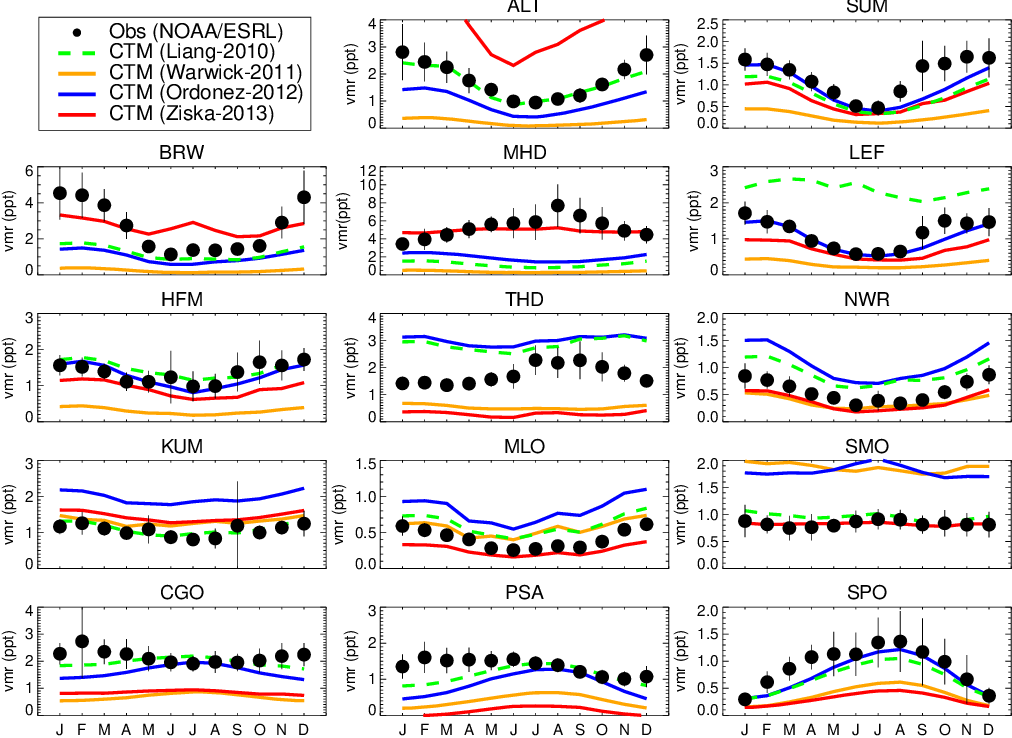
\includegraphics[width =0.7\linewidth]{Appendix/images/Hossaini2013_fig5_bromoform.png}
    \caption{Comparison of monthly mean mixing ratio (ppt) of $\chem{CHBr_3}$ output from \cite{Liang2010}, \cite{ziska}, warwick 2011, ordonez 2012}
    \label{fig:Hosaini_fig5}
\end{figure}

\begin{figure}
    \centering
    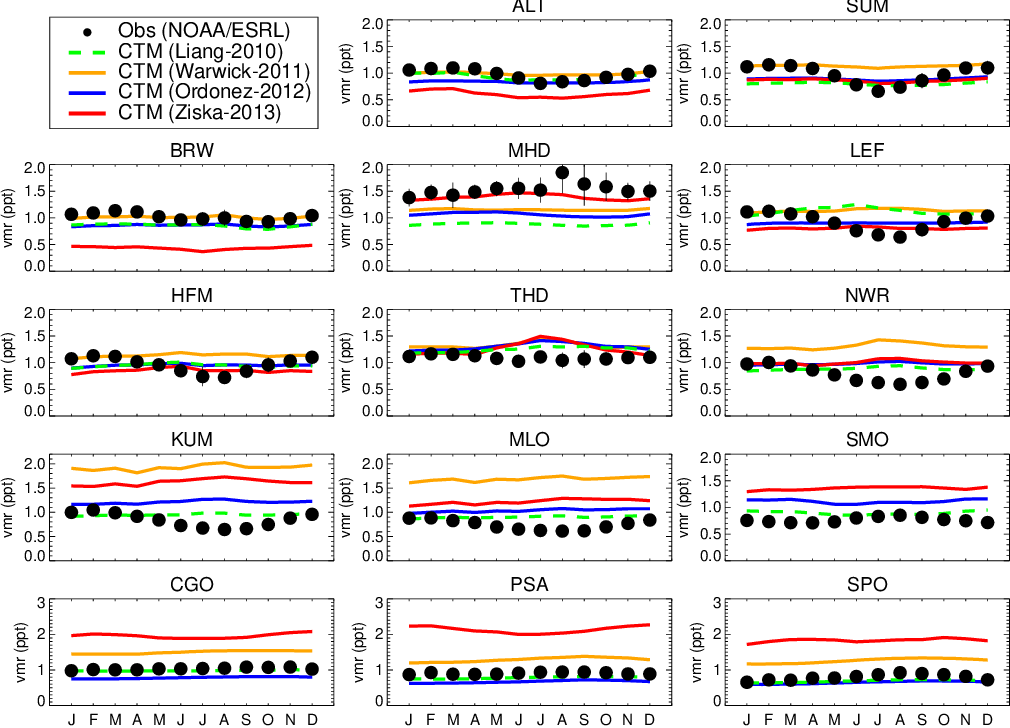
\includegraphics[width =0.9\linewidth]{Appendix/images/Hossaini2013_fig6_ch2br2.png}
    \caption{Comparison of monthly mean mixing ratio (ppt) of $\chem{CH_2Br_2}$ output from \cite{Liang2010}, \cite{ziska}, \cite{Warwick2006} and \cite{Ordonez2012}. The figure is adapted from \cite{Hossaini2013}}
    \label{fig:Hosaini_fig6}
\end{figure}


\cleardoublepage

\chapter{EBAS and NOAA data}\label{app:ebas_noaa_data}


\section{Station data}

Some key information about the station data obtained from ebas (\cite{EBAS}) is listed in Table \ref{tab:ebas_noaa_data_taken}. 

\begin{table}[ht]
\centering
\resizebox{14cm}{!}{%
\begin{tabular}{|lllllll|}
\hline
\textbf{Station}  & \textbf{Variable}  & \textbf{Temporal res.} & \textbf{Timzone} & \textbf{Unit}  & \textbf{Instrument type} & \textbf{Year} \\ \hline
Alert            & $\chem{O_3}$ & 1h           & UTC              & $\mu$gm$^{-3}$  & uv\_abs                  & 2001               \\
Alert            & \chem{Cl}    & 1w           & UTC              & $\mu$gm$^{-3}$  & high\_vol\_sampler       & 2001, 2013         \\
Alert            & \chem{Br}    & 1w           & UTC              & $\mu$gm$^{-3}$  & high\_vol\_sampler       & 2001, 2013         \\
Barrow           & $\chem{O_3}$ & 1h           & UTC              & nmol/mol        & uv\_abs                  & 2001, 2013, 2018   \\
Eureka           & $\chem{O_3}$ & 1h           & UTC              & nmol/mol        & uv\_abs                  & 2018               \\
Summit           & $\chem{O_3}$ & 1h           & UTC              & nmol/mol        & uv\_abs                  & 2001, 2013, 2018   \\
Tiksi            & $\chem{O_3}$ & 1h           & UTC              & nmol/mol        & uv\_abs                  & 2013, 2018         \\
Villum           & $\chem{O_3}$ & 1h           & UTC              & $\mu$gm$^{-3}$  & uv\_abs                  & 2013               \\
Villum           & \chem{Cl}    & 1w           & UTC              & $\mu$gm$^{-3}$  & filter\_3pack            & 2013, 2017         \\
Villum           & \chem{Br}    & 1w           & UTC              & $\mu$gm$^{-3}$  & filter\_3pack            & 2017               \\
Zeppelin         & $\chem{O_3}$ & 1h           & UTC              & $\mu$gm$^{-3}$  & uv\_abs                  & 2001, 2013, 2018   \\ \hline
\end{tabular}
}
\caption{Key information about data taken from the different stations (\cite{EBAS}). The arithmetic mean value was used from all datasets. The temporal resolution, timezone and unit were given by each dataset. uv\_abs refers to the ultraviolet absorption method (For more information, see e.g. \cite{Galbally2013}). high\_vol\_sampler and filter\_3pack. The years were chosen according to when the model simulations were planned}
\label{tab:ebas_noaa_data_taken}
\end{table}


\section{Ozonosonde data}

Ozonosonde measurements from Summit, Greenland, was obtained from \cite{NOAA} for the year 2013. The ozonosonde measures ozone by using an Electrochemical Concentration Cell Ozonosonde (For more information, visit \cite{ESRL}).  

\cleardoublepage

\chapter{Running the CTM3}\label{app:running_CTM3}

\cleardoublepage

\chapter{Turning Off the Stratosphere}\label{app:turning_off_the_stratosphere}

In order to save CPU time and avoid conflicts regarding the use of stratospheric methyl bromide ($\chem{CH_3Br}$) as a designated species for $\chem{CHBr_3}$ and $\chem{CH_2Br_2}$ (explained further in Section \ref{sec:oceanic_emissions}), the stratosphere was turned off. This is performed by modifying the following scripts: 

\section{Makefile}\label{subsubsec:makefile}

\texttt{Makefile} is the file that sets the user options for the CTM3. The resolution was either set to \texttt{HTWO} (2.25$^o$x2.25$^o$) or \texttt{HFOUR} (4.5$^o$x4.5$^o$). The following modules were also turned on or off (information about the different modules can be found in \cite{SovdeManual}):

\begin{itemize}
    \item \texttt{OSLOCHEM}: compilation with Oslo chemistry/physics, \textbf{turned on}
    \item \texttt{TROPCHEM}: compilation with Oslo tropospheric chemistry, \textbf{turned on}
    \item \texttt{STRATCHEM}: compilation with Oslo stratospheric chemistry, \textbf{turned off}
    \item \texttt{SULPHUR}: sulfur scheme, \textbf{turned on}
    \item \texttt{BCOC}: black carbon/organic matter scheme, \textbf{turned off}
    \item \texttt{NITRATE}: nitrate scheme (\texttt{SALT} and \texttt{SULPHUR} is required), \textbf{turned on}
    \item \texttt{SEA SALT}: sea salt scheme, \textbf{turned on}
    \item \texttt{DUST}: dust scheme, \textbf{turned off}
    \item \texttt{SOA}: secondary organic aerosols scheme, \textbf{turned off}
    \item \texttt{E90}: applies e90 tracer for STE flux calculations and produces the troposphere, \textbf{turned off}
    \item \texttt{LINOZ}: applies Linoz $\chem{O_3}$ for STE calculations (not set up yet to replace stratospheric chemistry in the Oslo CTM3), \textbf{turned off}
    \item \texttt{M7}: not implemented \textbf{turned off}
\end{itemize}


\section{Tropospheric Chemistry Parameters - \texttt{cmn\_size.f90}}\label{subsubsec:cmn_size}


The tropospheric chemistry parameters were adjusted in \texttt{cmn\_size.f90} in order to be able to include some of the originally stratospheric tracers without including the stratosphere. This was only done for the \texttt{bromine\_explosion}-branches (An overview of the branches can be seen in Section \ref{sec:code_availability}). 

\medskip

The non-transported species (\texttt{NPAR\_TROP}) were adjusted from 39 to 54 and the transported species (\texttt{NOTRPAR\_TROP}) were adjusted from 7 to 8 leaving the following amount of chemical parameters:

\begin{itemize}
    \item \texttt{TROPCHEM}: 54 transported, 8 non-transported
    \item \texttt{SULPHUR}: 5 transported
    \item \texttt{NITRATE}: 5 transported
    \item \texttt{SEA SALT}: 8 transported
\end{itemize}

The numbers of transported- and non-transported species must match the number of these species in the tracer list (see Section \ref{subsubsec:tracer_list}) 


\section{Component Output - \texttt{gmdump3hrs.f90}}\label{subsubsec:gmdump}

In the module \texttt{gmdump3hrs.f90}, selected tracer components are printed every hour. In this module, the tracer output was adjusted to dump 19 components instead of 7. To be able to do this, the components must be declared as "transported" in the tracer list (Described in Section \ref{subsubsec:tracer_list}) and in \texttt{cmn\_size.F90} (Described in Section \ref{subsubsec:cmn_size}).


\cleardoublepage

\chapter{Pre-Industrial Run}\label{app:PI_run}


The model was run with pre-industrial emissions, taken as the year 1850 in this thesis (\cite{IPCCchapter8}). In order to set up the CTM3 for this, a few steps has to be changed. Keep in mind that the approach was hard-coded in order to avoid having to make a 9 years spin up in the restart-file (due to the atmospheric lifetime of methane). 

\medskip

The tracer list,  \texttt{Ltracer\_emis\_ceds17\_1850\_megan.d}, was set for 1850. 

\medskip

In \texttt{ch4routines.f90}, the subroutine \texttt{ch4surface\_scale\_hymn} was activated along with \texttt{ch4surface\_hymn}, allowing scaling of the methane-surface field with 1850 values, taken as 808.25 ppm (value suggested by \cite{RagnhildPersonal}). The scaling was hard-coded to this value. 

\medskip

The subroutine \texttt{set\_ch4\_stt} (also in \texttt{ch4routines.f90}) was activated from \texttt{pmain.f90} to allow scaling of the entire field (lev, lon and lat) (not only the surface field). 

\cleardoublepage

\chapter{Chemical Unit Conversion}

The following appendix contains the conversion procedures concerning the CTM3 output as well as the conversion of station data to a mass mixing ratio. When analysing atmospheric data such as gases, it is most appropriate to use the mixing ratio (mol mol$^{-1}$), or mole fraction, as it is not dependent on pressure and temperature as the concentration (mol m$^{-3}$) is. It is defined as the ratio of the amount (or mass) of the substance in a given volume to the total amount (or mass) of all constituents in that volume (\cite{SeinfeldSpyros}). 

\medskip

The first section contains the formulas applied to the CTM3 data and the EBAS/NOAA data. The second section contains the \acrfull{cdo} procedure, which is a procedure for processing \acrshort{netcdf}-files. 

\section{Chemical Unit Conversion}

\subsection{Oslo CTM3}\label{sec:unit_conversion_CTM3}

The CTM3 data used were given in either monthly averages or tropospheric tracers (3-hour outputs). The monthly averages have units kg of species, and the 3-hour outputs have units g m$^{-3}$. 

\medskip

To obtain the mixing ratio from the monthly averages, the following was applied:

\begin{equation}
    \chem{X_{VMR}} = \frac{\chem{M_{air}}}{\chem{M_{X}}}\frac{\chem{X_{kg}}}{\chem{air_{kg}}}
    \label{eq:vmr_monthly_avg}
\end{equation}

In which $\chem{X_{VMR}}$ is the volume mixing ratio of the species, $\chem{M_X}$ and $\chem{M_{air}}$ are the molecular masses of the species of interest and air. $\chem{X_{kg}}$ and $\chem{air_{kg}}$ are the output data from CTM3 in kg of species. 

\medskip

In order to change the units of the tropospheric tracers (3-hour output), the following was performed: 

\begin{equation}
    \chem{X_{VMR}} = \frac{\chem{M_{air}}}{\chem{M_{X}}}\frac{\chem{X_{ g/cm^{3}}}}{\chem{\rho_{air}}}
    \label{eq:vmr_trop_tracer}
\end{equation}

In which  $\chem{X_{\mu g/m^{3}}}$ is the concentration of the species and $\chem{\rho_{air}}$ is the density of air (in $\mu g/m^{3}$). These are the output data from CTM3.


\subsection{EBAS/NOAA}\label{sec:unit_conversion_EBASNOAA}

The EBAS and NOAA data were provided in units $\mu g m^{-3}$, and were thus changes by: 

\begin{equation}
    \chem{X_{VMR}} = \frac{\chem{M_X}}{\chem{M_{air}}}\frac{\chem{X_{\mu g/cm^{3}}}}{\chem{\rho_{air}}}
\end{equation}

Density of air was taken as 1.204 kgm$^{-3}$ (at 293.15 K). This density was used in the EBAS-database files to convert


\section{Unit Conversion Using cdo}\label{sec:cdo}

The \acrshort{cdo}-software is a collection of operators for standard processing of climate and forecast data (\cite{cdo}). CDO is ideal for processing of large \acrshort{netcdf} datasets. 


\medskip

The \acrshort{cdo}-scripts were adapted from scripts provided by \cite{StefaniePersonal}. 



\begin{itemize}
    \item Load cdo by \texttt{module load cdo}
    \item \texttt{chmod +x "cdo file"} if there has been changes
    \item \texttt{./"cdo file" "Full path"} 
\end{itemize}

\cleardoublepage


\chapter{Figures}
%\addcontentsline{toc}{chapter}{Appendix B: Additional figures}
\cleardoublepage
